\documentclass[a4paper,10pt,onecolumn,oneside,titlepage]{article}

\usepackage[utf8]{inputenc}
\usepackage[spanish]{babel}
\usepackage{graphicx}
\usepackage[left=2cm,right=2cm,top=2cm]{geometry}
\usepackage{float}
\usepackage{rotating}
\usepackage{color}
\usepackage{xcolor}
\usepackage{listings}
\usepackage{caption}
%\usepackage{lscape}

\renewcommand{\baselinestretch}{1.5}
\addtolength{\parindent}{0pt}
\addtolength{\parskip}{\baselineskip}
\bibliographystyle{ieeetr}

\lstset{
% general command to set parameter(s)
basicstyle=\ttfamily, % print whole listing small
keywordstyle=\color{black}\bfseries\underbar, % underlined bold black keywords
identifierstyle=, % nothing happens
commentstyle=\color{white}, % white comments
stringstyle=\ttfamily, % typewriter type for strings
showstringspaces=false % no special string spaces
}

\title{Memoria Final - Aprendizaje Automático}
\author{Ignacio Robledo Rosell \\
				g990406}
\date{10 de Septiembre de 2012}

\includeonly{
	introduccion,
	metodologia,
	resultados,
	discusion,
	conclusiones
}

\begin{document}

\maketitle

\tableofcontents

\section{Introducción.}

La Asociación de Veteranos Paralíticos de EEUU \cite{PVA} es una organización sin ánimo de lucro cuyo objetivo principal es mejorar la vida de soldados heridos gravemente durante el desarrollo de su profesión. Según ellos mismos describen en su sitio web oficial en internet, buscan proporcionar los medios y alternativas suficientes para que estas personas puedan desarrollar su libertad e independencia dentro de las limitaciones impuestas por su estado físico.

Como organización sin ánimo de lucro, todos los fondos que utiliza en sus diferentes programas, son recaudados a partir de las aportaciones realizadas por los ciudadanos de los EEUU. La asociación cuenta con una importante base de datos de donantes que han realizado sus aportaciones en el pasado. Realiza una intensa actividad de comunicación sobre los mismos para mantenerlos informados de los nuevos programas, de las nuevas actividades y de este modo incentivar la aportación de nuevas donaciones.

Todas estas actividades de comunicación son caras y el presupuesto que tiene la asociación es bastante reducido. Por ello ha decidido que quiere invertir en los mecanismos necesarios para realizar una óptima y eficiente gestión de ese presupuesto, maximizando los resultados obtenidos del mismo.

A lo largo de este documento se detalla el desarrollo de algunas herramientas de inteligencia de negocio que permitirán a la asociación seleccionar y priorizar los donantes presentes en la base que tienen mayor potencial para realizar una nueva donación.

Este ejercicio fue propuesto en el ámbito del concurso KDD CUP \cite{KDD-CUP} organizado por el grupo de DataMining de la organización ACM \cite{SIGKDD-ACM} en 1998. Todos los conjuntos de datos necesarios están a libre disposición en la dirección web del KDD Contest \cite{KDD-CUP-1998}.
\section{Metodología.}

A lo largo de esta sección se detalla la metodología empleada para el desarrollo de los diferentes clasificadores. La metodología escogida sigue la filosofía del estándar de la industria CRISP-DM obviando por supuesto la fase de despliegue y puesta en producción de los modelos.

\subsection{Entendimiento del problema / negocio.}

A lo largo de esta fase se ha revisado el contenido del sitio oficial en internet de la PVA para entender bien la labor realizada por la asociación, la labor de los donantes, los diferente medios existentes para realizar donaciones, etc. 

También se ha revisado el contenido del fichero \emph{cup98doc.txt} que se encontraba disponible junto los ficheros de datos dentro de la página de descarga del KDD Contest \cite{KDD-CUP-1998} del grupo SIG-KDD (ACM) \cite{SIGKDD-ACM}, con una breve descripción del contexto del problema.

\subsection{Auditoría de datos.}

La fase de auditoría de datos ha sido la más extensa en tiempo dentro de todo el proyecto. En un primer momento se trato de realizar esta fase con la herramienta Weka \cite{WEKA} propuesta como herramienta de trabajo al comienzo del proyecto. Finalmente, tuvo que descartarse el uso de esta herramienta para esta fase, dado que presenta bastantes problemas de rendimiento y eficiencia para el trabajo con conjuntos de datos relativamente grandes. En este caso, a pesar de no contar con un conjunto de datos excesivamente grande, la herramienta Weka no conseguía desenvolverse con facilidad.

Se estudiaron diversas alternativas de trabajo para poder auditar y manipular los datos. Una de las opciones estudiada fue cargar los ficheros en tablas de un servidor de base de datos MySQL y manipularlas a través del propio lenguaje SQL. Aunque esta opción funcionaba y desde el punto de vista del rendimiento era bastante óptima, el lenguaje SQL no se mostraba como un lenguaje cómodo para el análisis estadístico.

Tras revisar que otras opciones existentes había en el mercado se opto por realizar toda la fase de auditoría y todas las fases posteriores de manipulado y preparación de la información previas a la fase de modelado con la herramienta R \cite{R}. R es un software de libre distribución para el tratamiento estadístico y la generación de gráficos por ordenador. Funciona en diversas plataformas UNIX y en el entorno Windows. Esta dotado de gran cantidad de utilidades y herramientas que facilitan el análisis estadístico y cuenta con varios plugins y módulos adicionales para trabajar con grandes cantidades de información, como por ejemplo, BigMemory.
Finalmente, no fue necesario hacer uso de ninguno de estos plugins adicionales, y con las instrucciones y herramientas básicas se pudo proceder a realizar la auditoría.

Como resultado de esta auditoría se ha construido un documento Excel maestro que contiene todas las variables y la información básica de la auditoría: 

\begin{itemize}

\item{Tipo de variable: numérica o categórica.}
\item{Número de valores distintos para las variables categóricas.}
\item{Número de valores nulos. Porcentaje de valores nulos.}
\item{Número de valores blancos. Porcentaje de valores blancos.}
\item{Valor mínimo para las variables numéricas.}
\item{Valor máximo para las variables numéricas.}
\item{Valor medio para las variables numéricas.}
\item{Valor de la mediana para las variables numéricas.}

\end{itemize}

Debido al elevado número de variables con el que se trataba y la escasa experiencia manipulando los datos con la herramienta R y la curva de aprendizaje que supuso, se decidió sólo trabajar con los conjuntos de datos de la información detallada del cliente y las variables resumen de las campañas recibidas y las donaciones realizadas.

Se decidió prescindir del detalle de las campañas de los últimos 24 meses al encontrarse esta información resumida en las variables resumen de las campañas recibidas y se decidió prescindir también de la información del censo al tratarse de información generalista y no información de carácter individual que puede ser útil para completar modelos pero no como base o punto de partida para construir un modelo.

A continuación se muestra el contenido de la hoja excel para las diferentes variables analizadas:

\begin{figure}[H]
\begin{center}
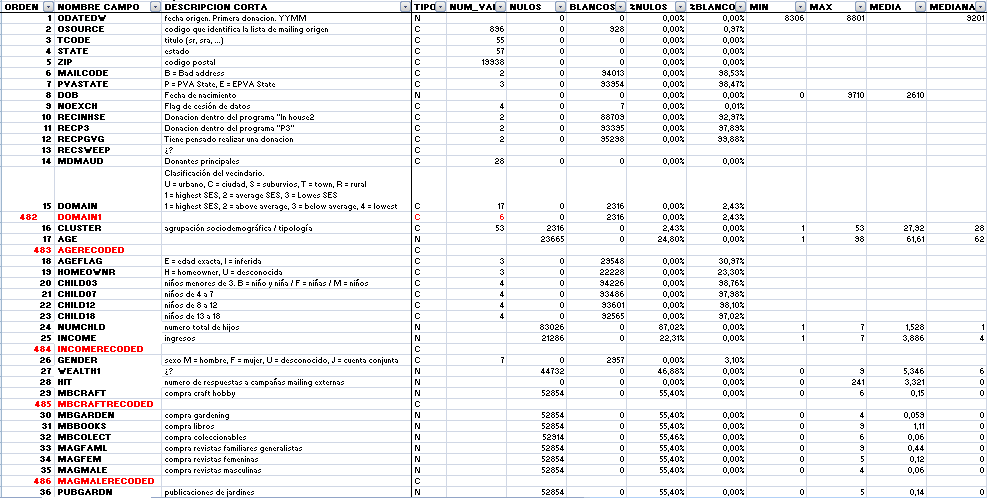
\includegraphics[width=0.95\textwidth]{img/audit1}
\caption{Captura de pantalla del excel de la auditoría de datos.}
\end{center}
\end{figure}

\begin{figure}[H]
\begin{center}
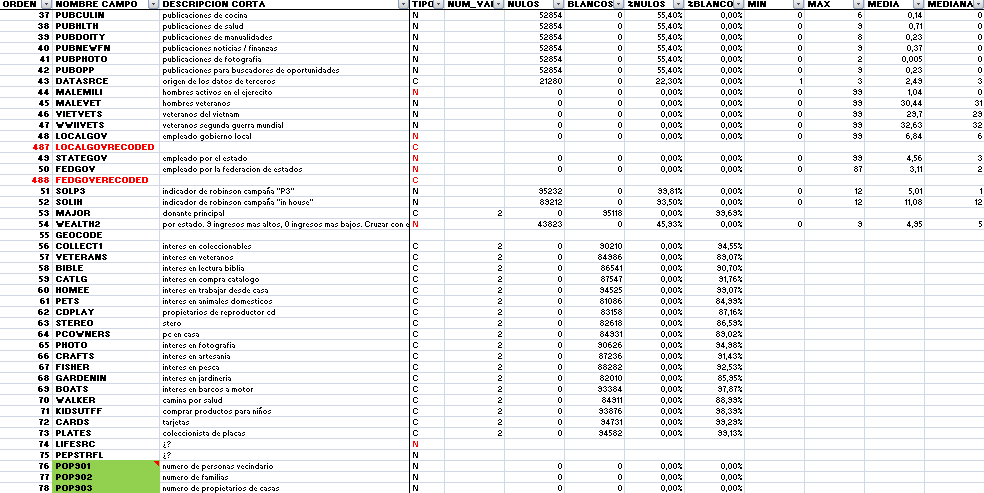
\includegraphics[width=0.95\textwidth]{img/audit2}
\caption{Captura de pantalla del excel de la auditoría de datos.}
\end{center}
\end{figure}

\begin{figure}[H]
\begin{center}
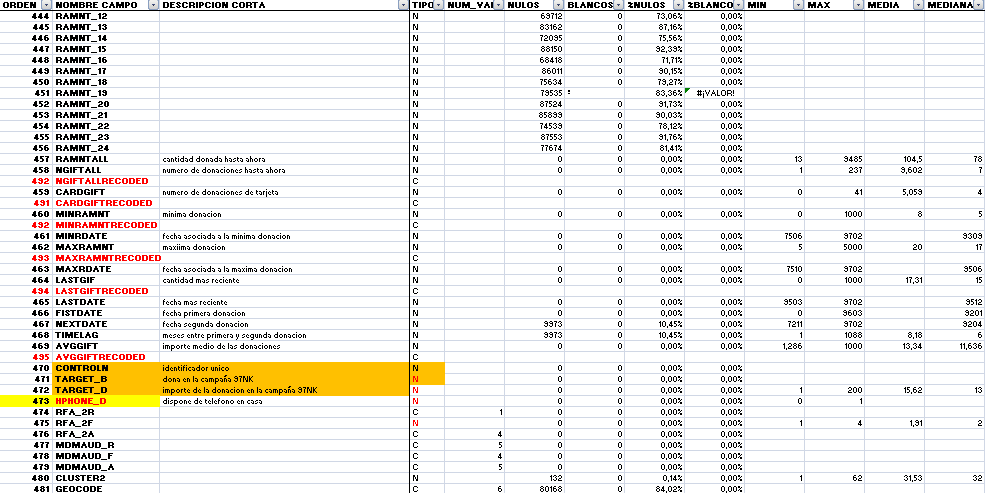
\includegraphics[width=0.95\textwidth]{img/audit3}
\caption{Captura de pantalla del excel de la auditoría de datos.}
\end{center}
\end{figure}

\subsection{Análisis univariante y recodificación de variables.}

Una vez realizada la auditoría se procedió a abordar la fase del análisis univariante donde se analiza la relación existente entre cada una de las variables de los conjuntos analizados y la variable objetivo del modelo que indica si un donante respondió positivamente al mailing enviado, realizando una donación.

Para realizar este análisis se procedió a automatizar una rutina en código R que permitiera realizar un test chi-cuadrado de cada una de las variables categóricas seleccionadas con la variable objetivo. Esta prueba permite medir el grado de asociación entre dos variables con un determinado nivel de confianza. El test se aplico de forma automática de dos formas diferentes: sin la corrección de Yates y con la corrección de Yates para seleccionar el valor adecuado del test en los casos en los que alguna combinación de valores de la variable objetivo y la variable a analizar presentan una frecuencia inferior a 5 casos.

Se completo el contenido de la hoja excel con el valor obtenido para el estadístico chi-cuadrado del test y con el p-valor asociado a este estadístico. A continuación se muestra el contenido de la hoja excel con los resultados del test:

\begin{figure}[H]
\begin{center}
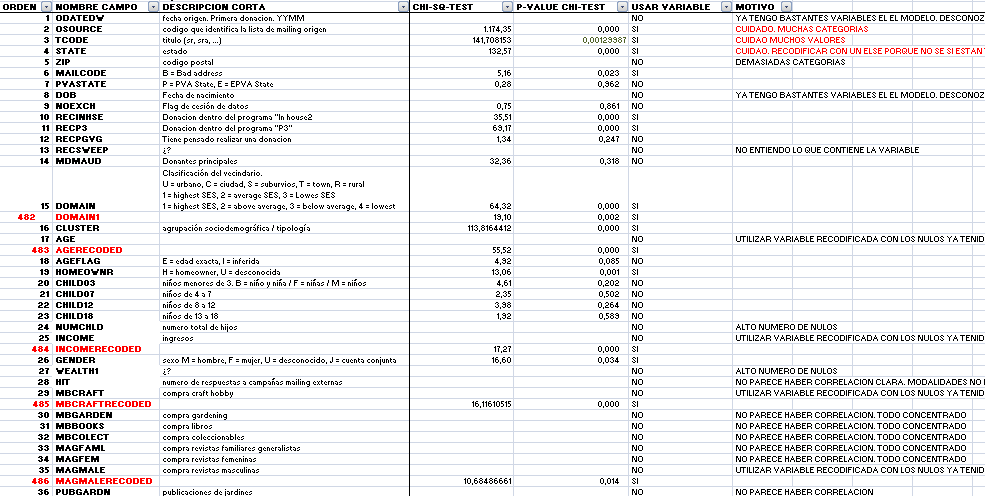
\includegraphics[width=0.95\textwidth]{img/univariante1}
\caption{Captura de pantalla del excel con los resultados del test chi-cuadrado y el p-valor asociado}
\end{center}
\end{figure}

Para las variables numéricas se procedió a automatizar una rutina en código R que partía en intervalos la variable y se analizaba el porcentaje de casos positivos de la variable target en cada uno de los intervalos. Este análisis permitía observar si el porcentaje de target era similar en todos los intervalos, de forma que no existe correlación entre la variable numérica y la variable target, o si por el contrario, según cambiabas de intervalo, el porcentaje de target era sensiblemente diferente.

\begin{figure}[H]
\begin{center}
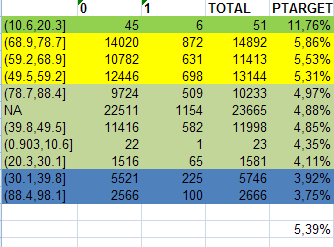
\includegraphics[width=0.4\textwidth]{img/cuantitativa1}
\caption{Captura de pantalla del excel con análisis de la correlación entre una variable numérica y la variable target}
\end{center}
\end{figure}

\begin{figure}[H]
\begin{center}
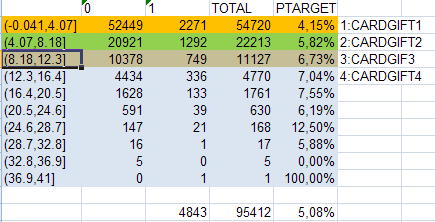
\includegraphics[width=0.4\textwidth]{img/cuantitativa2}
\caption{Captura de pantalla del excel con análisis de la correlación entre una variable numérica y la variable target}
\end{center}
\end{figure}

Con esta información se procedió a categorizar las variables numéricas que si mostraban una clara relación con la target. Sobre todo las variables que resumían el número de campañas recibidas y el número de donaciones realizadas. Sobre estas nuevas variables categóricas se volvió a realizar el test de la chi-cuadrado.

\subsection{Selección de variables.}

En la fase de selección de variables se establecieron varios criterios para limpiar la lista inicial de posibles variables candidatas y definir el conjunto final de trabajo. En concreto:

\begin{itemize}

\item{Variables con porcentaje de nulos o blancos superior al 20\%.}
\item{Valor del test de chi-cuadrado alto con un p-valor igual o inferior a 0,05.}
\item{Variable categórica con 15 o menos posibles valores diferentes. Priorizando variables con 5 valores o menos.}
\item{Variable numérico que guarda correlación con la variable target. Se incluye la variable numérica y la variable categórica recodificada.}

\end{itemize}

Las variables que contenían nulos fueron recodificadas agrupando las categorías en función del porcentaje de target y los nulos fueron agrupados con alguna de las categorías o se creo una categoría propia para ellos.

A continuación se muestra el listado final de variables seleccionado para entrenar los diferentes modelos:

\begin{figure}[H]
\begin{center}
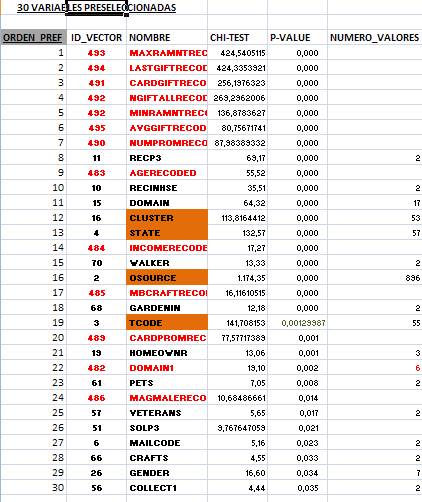
\includegraphics[width=0.7\textwidth]{img/seleccion}
\caption{Selección de variables para utilizar en la fase de modelado.}
\end{center}
\end{figure}


\subsection{Balancear ficheros de entrenamiento.}

Los conjuntos de entrenamiento y validación con las variables seleccionadas y recodificadas presentaban una gran descompensación en cuanto al número de casos positivos y casos negativos de la variable target. Esto impide que algunos algoritmos de aprendizaje, especialmente en el caso de los árboles, aprendan correctamente, favoreciendo la clasificación completa de todos los casos como casos negativos. 

Para solventar esta situación se precedió a codificar en lenguaje R una rutina de sobremuestreo que permitiera equilibrar en los ficheros de entrenamiento el número de casos positivos y negativos de la variable target.

Con esta rutina se construyo un dataset de entrenamiento con 7.770 instancias, de las cuales, 3.885 positivas y 3.885 negativas.

\subsection{Construcción de los modelos.}

La fase de construcción de los modelos ha sido ejecutada siguiendo los mismos pasos para cada uno de los algoritmos identificados como algoritmos potenciales para construir los clasificadores:

\begin{itemize}

\item{Ejecución del algoritmo con todas las variables del fichero de entrenamiento.}
\item{Ajuste de los parámetros del algoritmo y ejecución con todas las variables hasta encontrar configuración adecuada del mismo.}
\item{Ejecuciones con diferentes selecciones de variables hasta encontrar conjunto óptimo de variables, considerando óptimo, como el algoritmo que proporciona mejores resultados sobre el conjunto de entrenamiento a través de un proceso de cross validation con 10 conjuntos.}
\item{Selección de los dos o tres modelos con mejores resultados de clasificación para utilizarlos en la última etapa de validación.}

\end{itemize}

Se ha construido una hoja excel por cada algoritmo donde se puede ver la secuencia de variables utilizadas y los resultados sobre el conjunto de entrenamiento. Estas hojas están detalladas en la siguiente sección del documento.

\subsection{Validación de los modelos.}

Una vez seleccionados los dos o tres modelos con mejores resultados por algoritmo se ha contrastado la eficiencia de los mismos contra el fichero de validación para verificar que realmente no existe un sobreajuste sobre la muestra de entrenamiento y los resultados del clasificador son suficientemente estables. 

Con esta información se ha elaborado finalmente la lista de modelos potenciales para ser utilizados en las campañas reales.
\section{Resultados.}

\subsection{ID3.}

En los gráficos siguientes se muestran los 21 modelos diferentes que se construyeron combinando las diferentes variables para entrenar el modelo con el algoritmo ID3. En color verde están marcadas las variables utilizadas en cada modelo. En la primera de las dos filas inferiores se muestra el porcentaje de instancias del conjunto de entrenamiento clasificadas correctamente por el algoritmo.

En la segunda de las dos filas inferiores se muestra el porcentaje de target para los modelos potenciales seleccionados como candidatos para ser el clasificador referencia construido con el algoritmo ID3. Como puede apreciarse el modelo V0, con todas las variables introducidas, clasifica correctamente prácticamente todas las instancias del conjunto de entrenamiento pero presenta un gran sobreajuste sobre esos mismas instancias. Esto se refleja en los resultados sobre el conjunto de validación.

En este caso, el modelo de referencia sería el V3 o el V20.

\begin{figure}[H]
\begin{center}
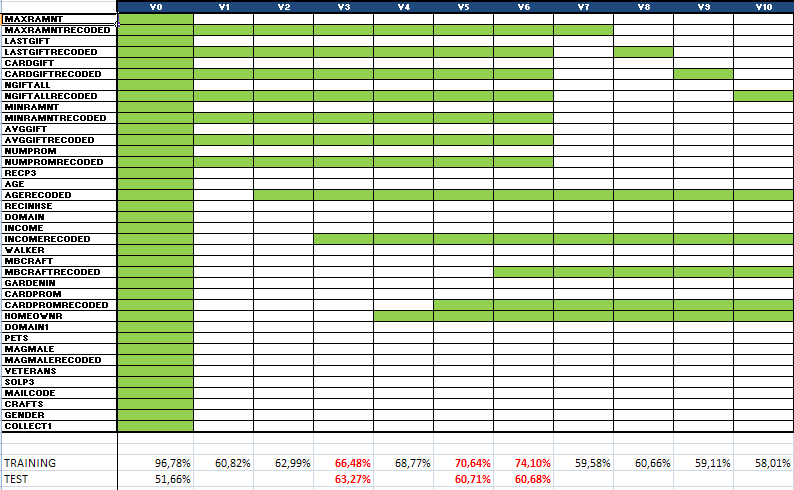
\includegraphics[width=0.9\textwidth]{img/id3-1}
\caption{Modelos construidos con el algoritmo ID3.}
\end{center}
\end{figure}

\begin{figure}[H]
\begin{center}
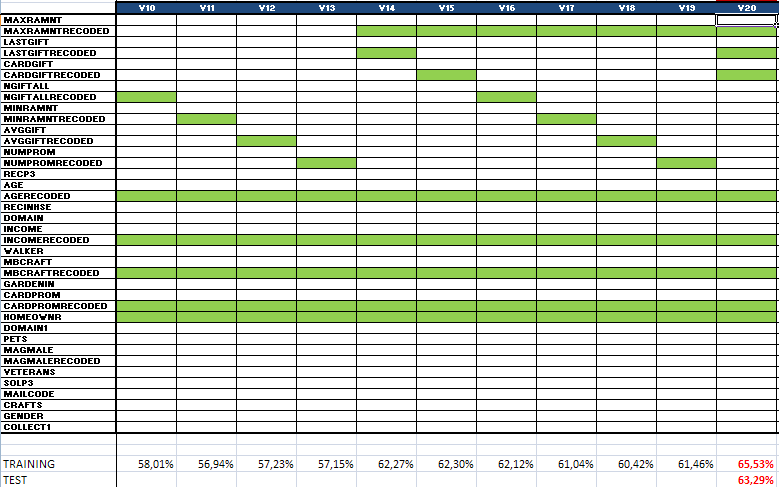
\includegraphics[width=0.9\textwidth]{img/id3-2}
\caption{Modelos construidos con el algoritmo ID3.}
\end{center}
\end{figure}

\subsection{J48.}

A continuación se muestra la información de los diferentes modelos construidos con el algoritmo J48. En este caso los modelos de referencia son el V5 y el V11. Aunque resulte extraño, no ha sido posible mejorar los resultados obtenidos con el algoritmo ID3.

\begin{figure}[H]
\begin{center}
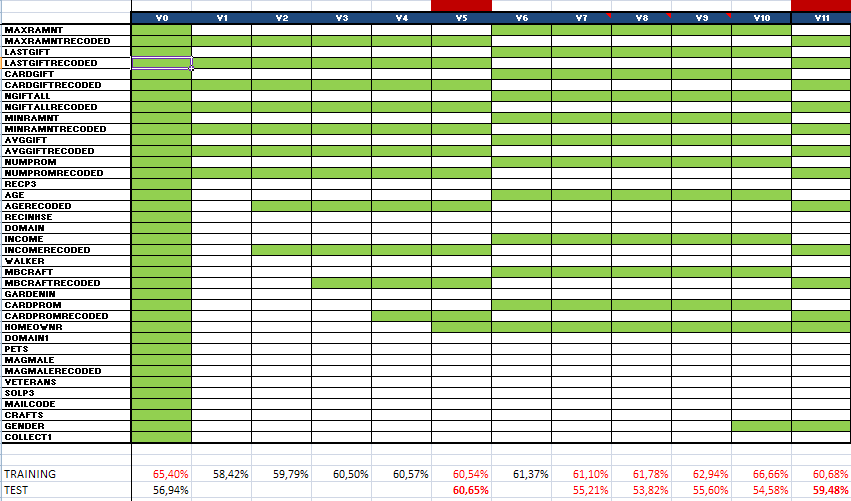
\includegraphics[width=0.9\textwidth]{img/j48-1}
\caption{Modelos construidos con el algoritmo J48.}
\end{center}
\end{figure}

Y esta es la tabla que muestra los diferentes parámetros probados previos al desarrollo de los modelos:

\begin{figure}[H]
\begin{center}
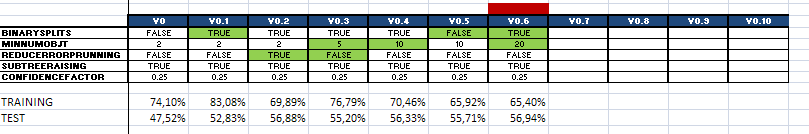
\includegraphics[width=0.9\textwidth]{img/j48-2}
\caption{Pruebas de los diferentes parámetros de configuración del algoritmo J48.}
\end{center}
\end{figure}

A continuación se muestra una captura de pantalla de la salida del algoritmo mostrada por la herramienta Weka:

\begin{figure}[H]
\begin{center}
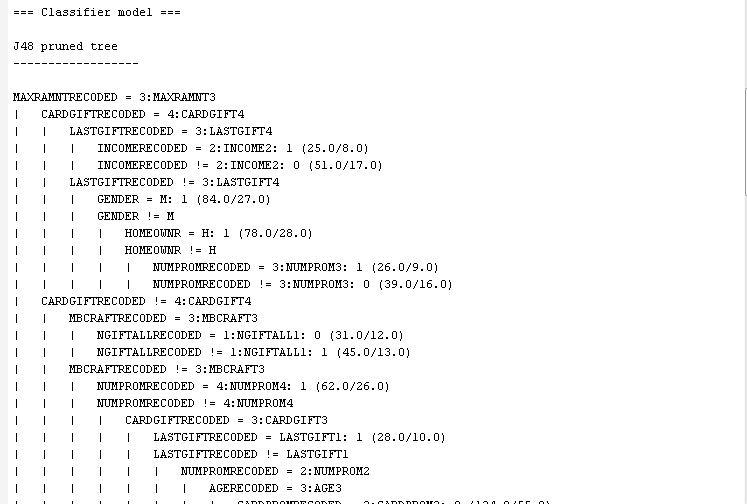
\includegraphics[width=0.9\textwidth]{img/j48-3}
\caption{Salida parcial de la herramienta WEKA del modelo construido con el algoritmo J48.}
\end{center}
\end{figure}

\subsection{M5P.}

La variable target es una variable discreta y no ha sido posible probar el algoritmo M5P.

\subsection{IB1.}

A continuación se muestra la información de los diferentes modelos construidos con el algoritmo IB1. En este caso no se ha seleccionado ningún modelo de referencia dado que todos los construidos tiene resultados muy por debajo de los obtenidos con los algoritmos anteriores.

\begin{figure}[H]
\begin{center}
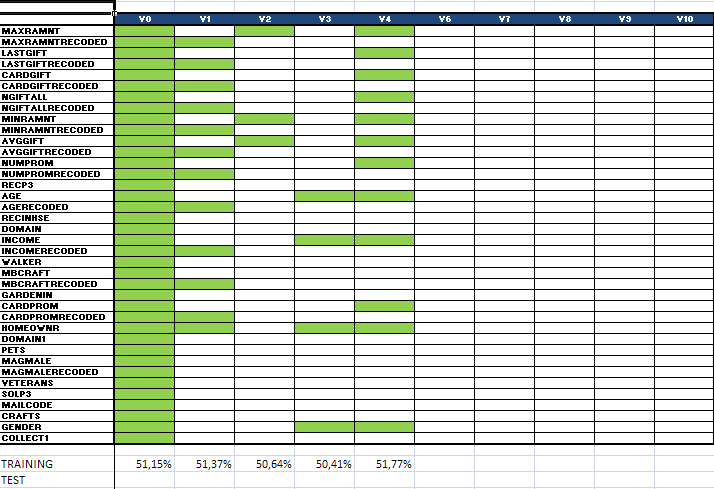
\includegraphics[width=0.9\textwidth]{img/ib1-1}
\caption{Modelos construidos con el algoritmo IB1.}
\end{center}
\end{figure}

\subsection{IBK.}

A continuación se muestra la información de los diferentes modelos construidos con el algoritmo IB1. En este caso no se ha seleccionado ningún modelo de referencia dado que todos los construidos tiene resultados muy por debajo de los obtenidos con los algoritmos anteriores.

\begin{figure}[H]
\begin{center}
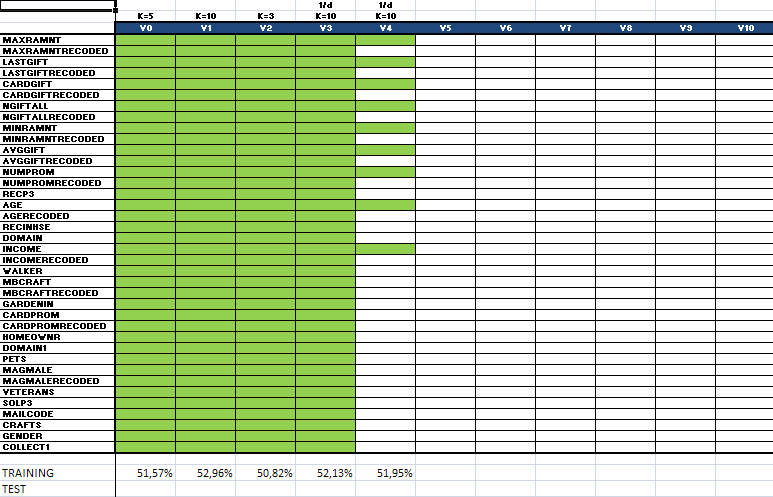
\includegraphics[width=0.9\textwidth]{img/ibk-2}
\caption{Modelos construidos con el algoritmo IBK.}
\end{center}
\end{figure}

Como puede observarse los mejores resultados se obtuvieron configurando el algoritmo con 10 vecinos y pesando por el inverso de la distancia.

A continuación se muestra una captura de pantalla de la salida del algoritmo mostrada por la herramienta Weka:

\begin{figure}[H]
\begin{center}
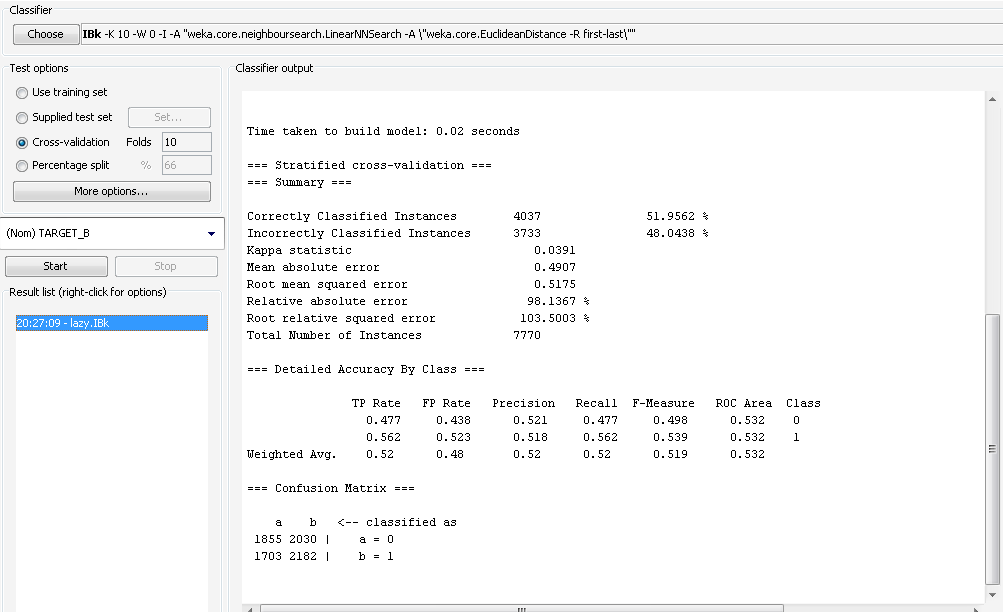
\includegraphics[width=0.9\textwidth]{img/ibk-1}
\caption{Salida parcial de la herramienta WEKA del modelo construido con el algoritmo IBk.}
\end{center}
\end{figure}

\subsection{Naive Bayes.}

A continuación se muestra la información de los diferentes modelos construidos con el algoritmo Naive Bayes. En este caso se ha seleccionado el modelo V2 como modelo de referencia aunque su <<performance>> es inferior a la obtenida con los algoritmos ID3 y J48.

\begin{figure}[H]
\begin{center}
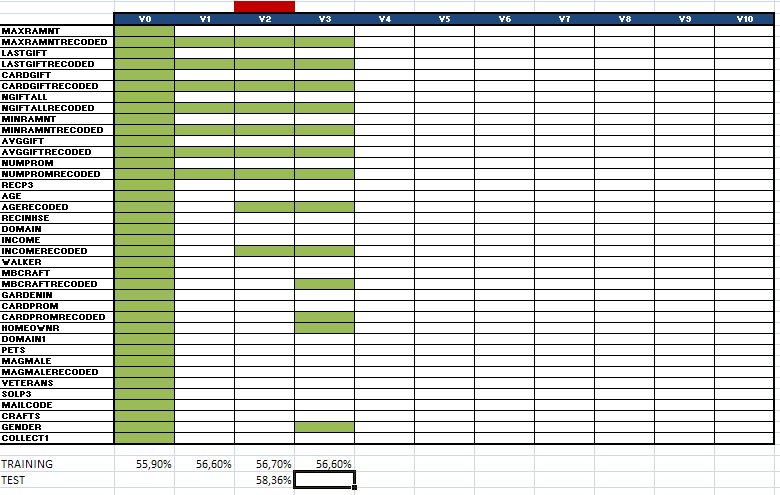
\includegraphics[width=0.9\textwidth]{img/nb-1}
\caption{Modelos construidos con el algoritmo Naive Bayes.}
\end{center}
\end{figure}

\subsection{TAN.}

A continuación se muestra la información de los diferentes modelos construidos con el algoritmo TAN. No se observa mejora respecto a los construidos con el algoritmo Naive Bayes y no se ha seleccionado ningún modelo de referencia.

\begin{figure}[H]
\begin{center}
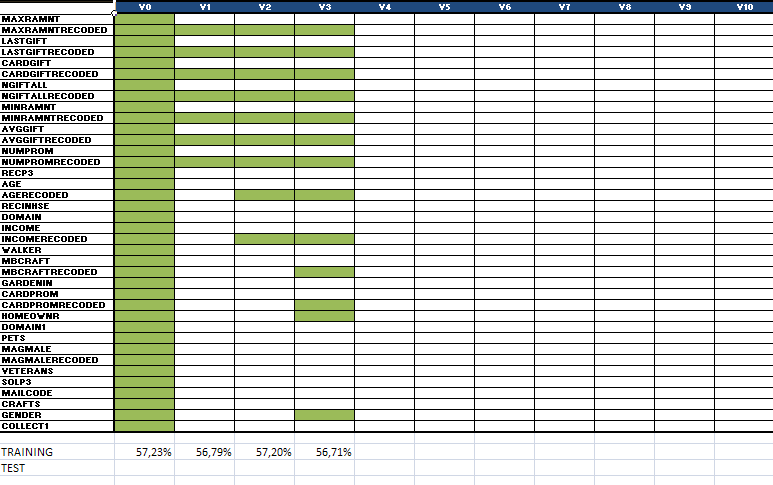
\includegraphics[width=0.9\textwidth]{img/tan-1}
\caption{Modelos construidos con el algoritmo TAN.}
\end{center}
\end{figure}

\subsection{Logistic.}

A continuación se muestra la información de los diferentes modelos construidos con el algoritmo Logistic. No se observa mejora respecto a los construidos con los algoritmos ID3 y J48 y no se ha seleccionado ningún modelo de referencia.

\begin{figure}[H]
\begin{center}
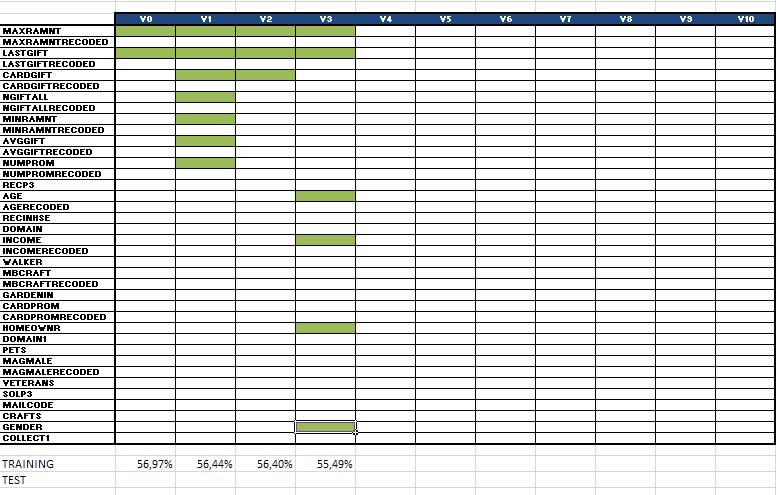
\includegraphics[width=0.9\textwidth]{img/logistic-2}
\caption{Modelos construidos con el algoritmo LOGISTIC.}
\end{center}
\end{figure}

Y una captura de pantalla de la herramienta WEKA mostrando las Betas asociadas a cada una de las variables del modelo V4:

\begin{figure}[H]
\begin{center}
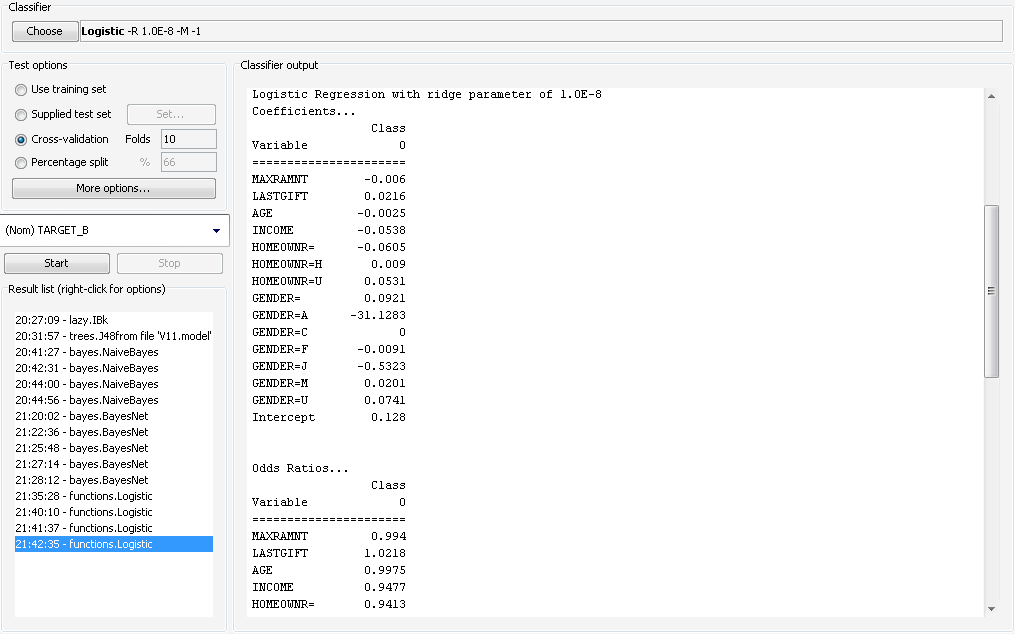
\includegraphics[width=0.9\textwidth]{img/logistic-1}
\caption{Salida parcial de la herramienta WEKA del modelo construido con el algoritmo LOGISTIC.}
\end{center}
\end{figure}

\subsection{JRIP.}

A continuación se muestra la información de los diferentes modelos construidos con el algoritmo JRIP:

\begin{figure}[H]
\begin{center}
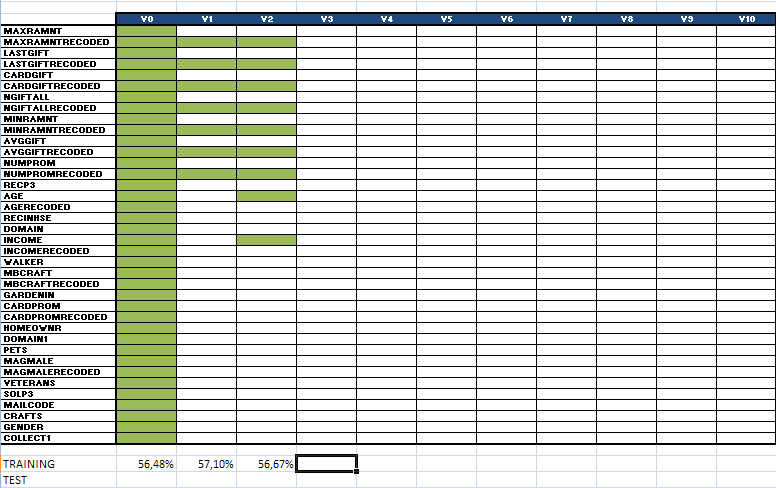
\includegraphics[width=0.9\textwidth]{img/jrip-2}
\caption{Modelos construidos con el algoritmo JRIP.}
\end{center}
\end{figure}

Y una captura de pantalla de la herramienta WEKA mostrando las reglas inducidas por el algoritmo:

\begin{figure}[H]
\begin{center}
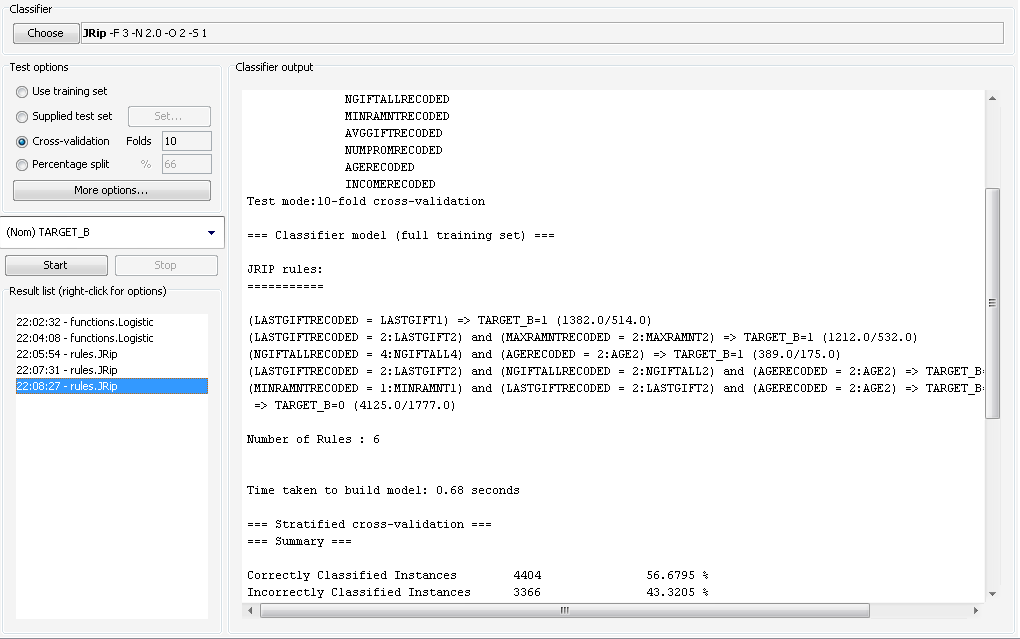
\includegraphics[width=0.9\textwidth]{img/jrip-1}
\caption{Salida parcial de la herramienta WEKA del modelo construido con el algoritmo JRIP.}
\end{center}
\end{figure}
\section{Discusión.}

A lo largo del artículo se han expuesto varios temas que merece la pena poner bajo discusión para evaluar su eficiencia a la hora de construir modelos analíticos como los mostrados en el mismo.

Una de las primera preguntas es, ¿merece la pena utilizar información agregada de los censos dentro de los modelos? Los censos contienen información que una vez publicada suele estar bastante desactualizada porque ha sido recogido hace bastante tiempo, ya que el proceso de recolección es muy costoso y laborioso en tiempo. La información de los censos es información agregada. ¿Qué validez tiene esta información al llevarla a nivel individual? ¿Realmente toda la gente que vive en una zona determinada comparte las mismas características? Todo esto lleva a concluir que el uso de información de censos y bases de datos de enriquecimiento agregadas puede utilizarse como refuerzo en la construcción de un modelo siempre que no supongan un excesivo coste extra tanto económico como en horas de desarrollo de los modelos.

Continuando con el tema de la información a utilizar en la construcción del modelo conviene preguntarse, ¿cómo de efectiva es la selección de variables por el criterio del test de la chi-cuadrado? ¿Es positivo poner una restricción del p-valor igual a 0,05 para realizar la selección o por ser tan estrictos se estarán dejando de lado variables importantes que pueden explicar significativamente una parte de los resultados del modelo? Tras el ejercicio desarrollado en el artículo se puede concluir que el criterio de 0,05 puede resultar demasiado estricto y perjudicar la posible eficiencia de los modelos a construir.

Un tercer punto de debate es la necesidad de balancear las muestras para que algunos algoritmos puedan aprender. ¿Hasta que punto las diferentes técnicas de sobremuestreo son eficientes? ¿Qué impacto tiene la pérdida de información que se produce? ¿Son eficientes las técnicas de sobremuestreo como la técnica SMOTE \cite{SMOTE}? Realmente no hay una respuesta clara y solo la experiencia y diferentes pruebas sobre cada conjunto de datos pueden ayudar a definir la mejor solución para cada problema.

Estas son las cuestiones más relevantes que pueden extraerse del artículo y que sólo la experiencia y la práctica con múltiples problemas y situaciones puede ayudar a encontrar las mejores y óptimas soluciones.



\section{Conclusiones.}

El desarrollo de este artículo ha permitido experimentar todas las etapas del desarrollo de modelos analíticos poniendo en práctica todo el contenido teórico estudiado durante la asignatura. Ha resultado un trabajo muy interesante y una gran aportación para reforzar los conceptos estudiados. 

También ha puesto de manifiesto que la herramienta Weka es un conjunto de algoritmos potentes de DataMining pero dista mucho de ser una herramienta útil y utilizable en un entorno productivo empresarial. Los problemas para manejar grandes cantidades de información y los estrictos formatos de los conjuntos de datos que necesita para realizar las validaciones de los diferentes modelos la convierten en una herramienta bastante improductiva que genera grandes demoras y pérdidas de tiempo en el desarrollo de modelos analíticos.

Para ello existen otras herramientas en el mercado para un uso intensivo profesional, como SAS Enterprise Miner e IBM SPSS Modeler que probablemente solucionen parte de las dificultades encontradas con el software WEKA con la contrapartida del alto coste económico de las licencias necesarias.

\newpage \bibliography{references}
\newpage \listoffigures
%\listoftables

\end{document}
